\section{Life Cycle}

\begin{figure}[t]
\begin{center}
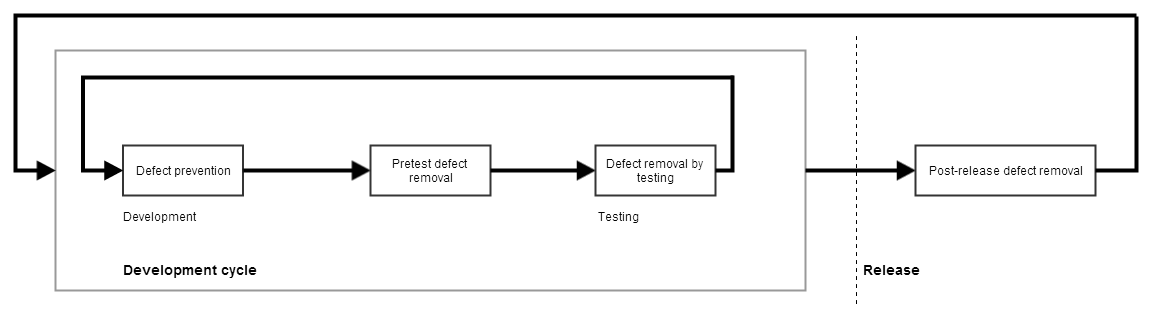
\includegraphics[width=1.0\textwidth]{image/quality_lifecycle.png}
\end{center}
\caption{Phases of software quality improvement in the software life cycle}
\label{fig:quality_life_cycle}
\end{figure}

A solid base for high quality is built with good specification, requirements and planning in the beginning of a project. When development begins, there should be ways to prevent as much defects as possible. As defects appear anyway, they should be detected and fixed as early as possible. Detecting the defects early lowers the effort needed to fix them. 

The hardest defects to remove are found in the requirements and design because testing and static analysis cannot find them. This is because these defects tend to be deficiency of features and errors of logic rather than errors in code. These defects are usually situated in the beginning of the life-cycle and thus require great effort to be removed. 

At some point, the project can initiate testing phase. Testing is used to systematically find defects in the software. Tests can be aimed to different areas of the software and the range of different tests used is dependent of the project. Big and critical projects should use comprehensive testing whereas smaller projects can get along with smaller amount of tests and lesser coverage.

Quality cannot be forgotten when the software is released. Because defect removal efficiency can never reach 100\%, there are always defects after the release. Some of those defects may have been found in the previous phases, but not removed, and other defects were unknown to the project team at the time of the release. Quality methods after the release should include detecting and removing defects and increasing the design for increasing the maintainability. With this range of methods divided to the software life-cycle, every project should choose the most appropriate methods to be used in the project in question.


TÄTÄ VOIS REFAKTOROIDA MUKAILEMAAN KUVAA~\ref{fig:quality_life_cycle} PAREMMIN

